\chapter{Metode Penelitian}

\section{Desain Penelitian}

\vspace{-.5cm}
\begin{figure}[h!]
  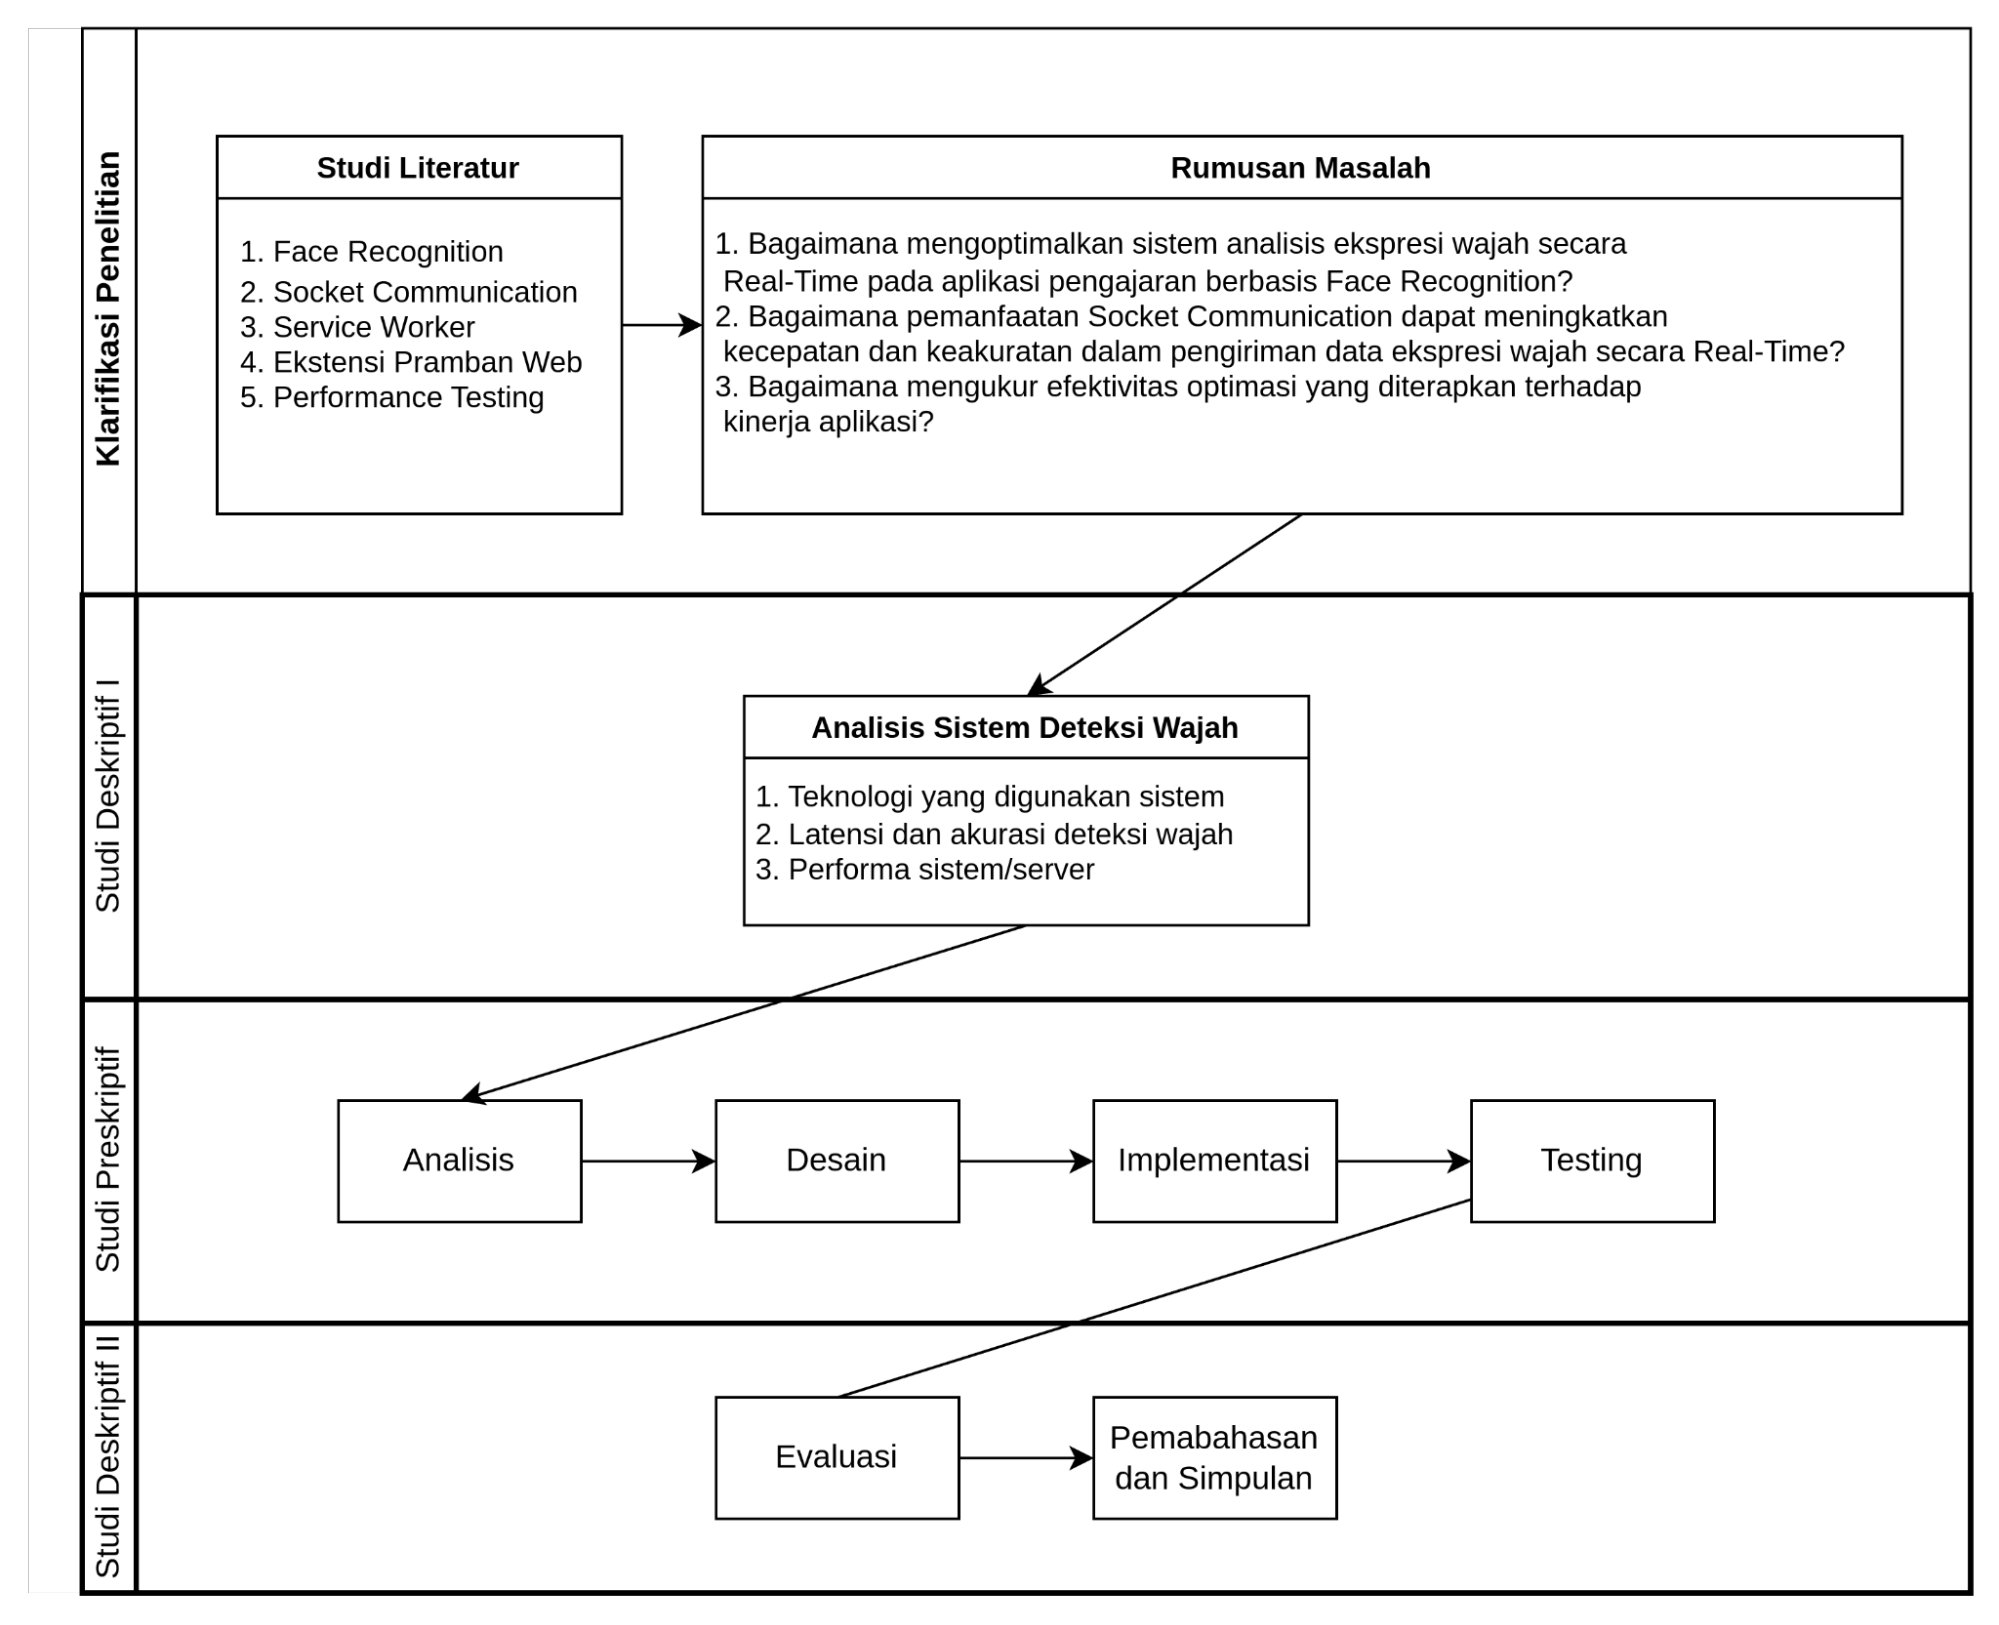
\includegraphics[
    width=14.5cm,
    height=13.5cm,
  ]{images/drm.png}
  \caption{Design Research Methodology (DRM)}
\end{figure}

Penelitian ini menggunakan pendekatan Design Research Methodology (DRM) untuk mengembangkan solusi teknis secara sistematis, bertujuan memahami dan mengoptimalkan sistem deteksi ekspresi wajah dalam aplikasi pengajaran real-time. Melalui DRM, penelitian berfokus pada tahapan identifikasi masalah, perancangan solusi, dan evaluasi hasil dalam konteks aplikasi pengajaran yang berbasis teknologi

\subsection{Klarifikasi Penelitian}
Tahap ini berfokus pada identifikasi masalah dan penentuan ruang lingkup secara spesifik. Pada tahap ini, penelitian bertujuan mengoptimalkan sistem deteksi ekspresi wajah guna meningkatkan performa dan keandalan aplikasi pengajaran real-time. Penelitian juga akan mengidentifikasi kebutuhan utama pengguna aplikasi, yaitu pengajar yang memerlukan data ekspresi siswa secara akurat dan tepat waktu. Untuk mendukung optimalisasi sistem, penelitian ini akan melakukan kajian pustaka yang lebih dalam terkait teknologi face recognition, socket communication, ekstensi pramban, dan pengujian performa.

\subsection{Studi Deskriptif I}
Pada tahap deskripsi, dilakukan pengumpulan data empiris guna memahami kondisi sistem yang ada serta tantangan yang dihadapi dalam penerapan deteksi ekspresi wajah pada aplikasi pengajaran. Penelitian akan melakukan analisis terhadap sistem eksisting atau konsep awal, seperti teknologi face recognition dan socket communication. Selain itu, studi kasus akan dilakukan pada aplikasi pengajaran real-time terkait, atau melalui prototipe awal, untuk memahami bagaimana deteksi ekspresi wajah dapat diimplementasikan secara optimal. Permasalahan teknis seperti latensi, akurasi deteksi wajah, dan performa sistem saat beban tinggi juga akan diidentifikasi pada tahap ini.

\subsection{Studi Preskriptif}
Pada tahap ini, penelitian akan merancang solusi untuk mengatasi masalah yang ditemukan pada tahap sebelumnya. Solusi ini difokuskan pada peningkatan performa deteksi ekspresi wajah melalui optimalisasi penerapan face recognition dan socket communication. Sistem yang dikembangkan akan mengikuti best practice developer untuk mencapai hasil optimal. Prototipe aplikasi yang dibangun akan memanfaatkan ekstensi pramban untuk pengumpulan data ekspresi wajah, service worker untuk caching data, dan socket communication untuk pengiriman data real-time. Metode evaluasi juga akan ditetapkan untuk mengukur kecepatan transmisi, akurasi deteksi ekspresi wajah, dan performa sistem secara keseluruhan.

\subsection{Studi Deskriptif II}
Pada tahap ini, sistem yang dikembangkan akan dinilai efektivitasnya dalam meningkatkan performa aplikasi pengajaran real-time. Pengujian performa akan dilakukan untuk mengukur kecepatan pengiriman data ekspresi wajah menggunakan socket communication dan keandalan face recognition di berbagai kondisi lingkungan dan jumlah pengguna. Evaluasi akan menilai keberhasilan optimasi dari segi akurasi, latensi pengiriman data, dan pengalaman pengguna. Analisis hasil dari pengujian ini akan membantu menentukan sejauh mana solusi ini dapat diterapkan pada skala yang lebih luas.

\section{Populasi dan Sampel}
Dalam penelitian ini, populasi yang ditargetkan adalah pengajar dan siswa yang menggunakan aplikasi pengajaran berbasis real-time. Pengambilan sampel akan dilakukan secara purposive sampling, di mana sampel terdiri dari pengajar yang menggunakan teknologi pengajaran serta siswa dari berbagai latar belakang yang bersedia berpartisipasi dalam pengujian aplikasi. Jumlah sampel akan ditentukan berdasarkan kebutuhan pengujian performa dan efektivitas sistem, dengan estimasi sekitar 10-20 partisipan. Pengajar berperan sebagai pengguna utama yang akan mengamati dan mengevaluasi ekspresi wajah siswa untuk mendukung proses pembelajaran, sementara siswa berperan dalam memberikan data ekspresi wajah yang akan dianalisis oleh sistem.

\section{Instrumen Penelitian}
Instrumen penelitian yang digunakan dalam penelitian ini meliputi beberapa komponen untuk mendukung pengumpulan data yang efektif. Pertama, prototipe aplikasi yang dikembangkan sebagai alat utama untuk mengimplementasikan sistem deteksi ekspresi wajah dan menguji performa sistem secara real-time. Kedua, kuesioner yang dirancang untuk mengukur persepsi pengguna, di mana pertanyaan dalam kuesioner ini akan mencakup aspek kepuasan pengguna terhadap keakuratan deteksi, dan pengalaman keseluruhan saat menggunakan aplikasi. Selain itu, pengujian teknis juga akan dilakukan untuk mengukur performa sistem menggunakan alat pengukuran latensi dan kecepatan, serta software analisis data untuk menganalisis hasil kuesioner dan pengamatan. Dengan instrumen-instrumen ini, diharapkan penelitian dapat memperoleh data yang komprehensif dan valid untuk mengevaluasi efektivitas sistem yang dikembangkan.

\section{Analisis Data}
Data hasil pengujian dan observasi dianalisis untuk menilai keberhasilan optimasi yang diterapkan. Analisis dilakukan secara kuantitatif untuk aspek performa teknis seperti latensi, kecepatan, dan akurasi, serta secara kualitatif untuk memahami persepsi pengguna terhadap aplikasi ini. Hasil analisis ini akan digunakan sebagai dasar untuk menarik kesimpulan serta memberikan rekomendasi bagi pengembangan sistem deteksi ekspresi wajah yang optimal pada aplikasi pengajaran berbasis real-time.
